\documentclass[11pt]{article}
\usepackage{tikz}
\usepackage{amsmath}
\usepackage[margin = 1.7 in]{geometry}
%opening
\title{An Exercise in Making Measurements and Propagating Error
\\ \large Finding the Area of a Tabletop and the Density of Metal Cylinder}
\author{Andreas Badea}
\date{\today}


\begin{document}

\maketitle 
\begin{center}
	\begin{tabular}{l r}
		Date Performed: & September 18, 2017 \\ % Date the experiment was performed
		Partners: & Emilio Foley \\ % Partner names
		& Mathew Huang \\
		Instructor: & Dr. Brad Miller % Instructor/supervisor
	\end{tabular}
\end{center}

\section{The Inevitability of Error}
Fundamentally, nearly all knowledge is in some sense erroneous. That is to say, that with the exception of tautologies, provable mathematical statements, and other knowledge a priori, the truth or falsity of a claim cannot be known with 100\% certainty. One may observe the occurrence of a certain event, say the release of an apple from a hand, one hundred times with the same result, that apple falling from that hand onto the floor, and it would be very reasonable to assume that when dropped for the one hundred and first time that apple would fall once again onto the floor. In fact, it would be rather unreasonable to assume the opposite. However, one cannot know for certain that the apple will not behave differently. Perhaps it will just float there in the air; Maybe it will fall up; Maybe all the previous falls were hallucinated and the apple never fell down in the first place. All of these assumptions would be unreasonable things to assume, but they remain possible. 

Modern science is based on empiricism. From an epistemological perspective, empiricism relies on two primary assumptions. Firstly, that similar objects in similar circumstances tend to behave in similar ways. And secondly, that one can reason about the behavior of objects by observing them. These seem like very reasonable assumptions to make. However, accepting these assumptions does not mean that we have to put 100\% of our faith into our observations. The scientists may realize that their observations may be flawed. However, their response is not to reject the observations, but instead to put their belief in the least flawed observations they can find. However, in order to be able to choose in which observation to believe, they must first be able to quantify just how flawed the observations could be.

One may estimate the most erroneous their observations could reasonably be and use this to figure estimate the quality of their findings. However, rarely is an interesting finding simply a matter of making an observation. Often calculations must be done regarding a series of differing observations to reach a meaningful conclusion. When estimating the error in a value one must make sure to bring the error of the initial observations along and consider them in judging the possible error in the conclusive observation.

As an exercise in judging the uncertainty in a given measurement, the area of tabletop and the density of a cylinder of metal were calculated and the estimated uncertainty in these respective values were found as well.


\section{Procedure}
\subsection{Area of a Table Top}
The length and width of a lab bench table top were found in order to find the area of that tabletop. 2 meter sticks were positioned on each end of the table such that the 10.00 cm mark was aligned with the edge of the table. Because the table was shorter than 180 cm in both length and width, the two meter sticks overlapped. A point was chosen on the 90.00 cm mark of one of the meter sticks and the distances from that point to each end were measured. This was done without removing the meter sticks. One of these distances was always 80.00 cm (90.00 cm mark - 10.00 cm initial starting position). This was done for both the length and width of the tables, and repeated 4 times each at different places on the table.
\begin{figure}[h]
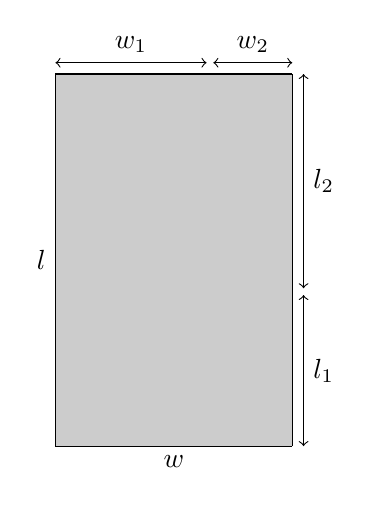
\begin{tikzpicture}[scale = 0.001cm]
\draw (0,0) -- node [below] {\(w\)} ++(105,0);
\draw (0,0) -- node [left] {\(l\)} ++(0,165);
\draw (0,165) -- (105,165);
\draw (105,0) -- (105,165);
\draw [<->] (110,0) -- node [right] {\(l_1\)} ++(0,67);
\draw [<->] (110,70) -- node [right] {\(l_2\)} ++(0,95);
\draw [<->] (0,170) -- node [above] {\(w_1\)} ++(67,0);\\
\draw [<->] (70,170) -- node [above] {\(w_2\)} ++(35,0);
\fill [opacity = 0.2] (0,0) rectangle (105,165);
\end{tikzpicture}
\centering
\caption{The length, \(l\), of the table was measured as a sum of 2 intermediary lengths, \(l_1\) and \(l_2\), one of which was fixed to 80.00 cm. In the same sense, the width \(w\) was a sum of \(w_1\) and \(w_2\), one of which was also fixed to 80.00 cm}
\end{figure}
\subsection{Density of a Metal Cylinder}
The height and diameter of a small metal cylinder of tin were measured three times with calipers. The cylinder of tin was then massed with a digital scale. 
\usetikzlibrary{shapes}
\begin{figure}[h]
	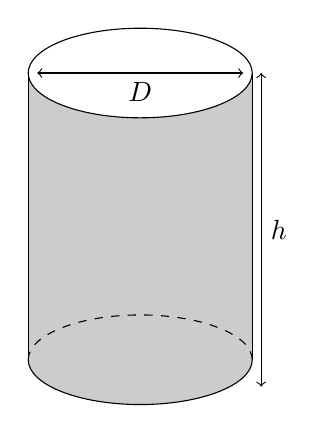
\begin{tikzpicture}[scale = 0.04cm]
	\draw (0,0) ellipse (1.25 and 0.5);
	\draw (-1.25,0) -- (-1.25,-3.2);
	\draw (-1.25,-3.2) arc (180:360:1.25 and 0.5);
	\draw [dashed] (-1.25,-3.2) arc (180:360:1.25 and -0.5);
	\draw (1.25,-3.2) -- (1.25,0);  
	\fill [opacity=0.2] (-1.25,0) -- (-1.25,-3.2) arc (180:360:1.25 and 0.5) -- (1.25,0) arc (0:180:1.25 and -0.5);
	\draw [<->] (1.15,0) -- node [below] {\(D\)}(-1.15,0);
	\draw [<->] (1.35,0) -- node [right] {\(h\)}(1.35,-3.5);
	\end{tikzpicture}
	\centering
	\caption{The height, \(h\) and the diameter, \(D\) of the tin cylinder were measured with calipers. The mass of the cylder was also taken with a digital scale}
\end{figure}



\section{Data}
\subsection{Width of Table}
The first and second intermediary widths of the tabletop were measured with meter sticks 4 times at a precision of \(\pm\)0.05 cm.
\begin{center}
	\begin{tabular}{|c|c|c|c|}
		\hline  
		\# & 1st Width (cm) & 2nd Width (cm) & Total Width (cm)\\
		\hline
		1 & 80.00 & 26.75 & 106.75 \\
		2 & 80.00 & 26.60 & 106.60 \\
		3 & 80.00 & 26.50 & 106.50 \\
		4 & 80.00 & 26.60 & 106.60 \\
		\hline
		\(\bar{x}\) & 80.00 & 26.61 & 106.61 \\
		\hline
		\(\delta_x\) & 0.05 & 0.10 & 0.11 \\
		\hline
	\end{tabular}
\end{center}
	The measurements of 1st width displayed no variance, as its length was fixed to 80.00 cm, however, it had an instrument uncertainty of 0.05cm. The 2nd width was not quite as constant, and had a sample standard deviation of 0.10 cm. This, being greater than the instrument uncertainty, represents the uncertainty in \( w_2 \). Assuming the two measurement are independent, of each other the uncertainty in their sum is 0.11 cm.
\subsection{Length of Table}
The first and second intermediary lengths of the tabletop were measured with meter sticks 4 times at a precision of \(\pm\)0.05 cm.
\begin{center}
	\begin{tabular}{|c|c|c|c|}
		\hline
		\# & 2st Length (cm) & 2nd Length (cm) & Total Length (cm)\\
		\hline
		1 & 80.00 & 82.80 & 162.80 \\
		2 & 80.00 & 82.65 & 162.65 \\
		3 & 80.00 & 82.65 & 162.65 \\
		4 & 80.00 & 82.50 & 162.50 \\
		\hline
		\(\bar{x}\) & 80.00 & 82.65 & 162.65 \\
		\hline
		\(\delta_x\) & 0.05 & 0.12 & 0.13 \\
		\hline
	\end{tabular}
\end{center}
	The 1st length also displayed no variance, as its length was also fixed to 80.00 cm, it had an instrument uncertainty of 0.05cm. The 2nd width was not held fixed and hence varied. It had a sample standard deviation of 0.12 cm. This, being greater than the instrument uncertainty, represents the uncertainty in \( l_2 \). Assuming the two measurement are independent of each other, the uncertainty in their sum is 0.13 cm.
\subsection{Diameter of the Cylinder}
The diameter of the cylinder was measured 3 times with callipers at a precision of \( \pm \)0.02cm.
\begin{center}
\begin{tabular}{|c|c|}
	\hline
	\# & Diameter of Cylinder (cm) \\
	\hline
	1 & 1.23 \\
	2 & 1.27 \\
	3 & 1.25 \\
	\hline
	\(\bar{x}\) & 1.25 \\
	\hline
	\( \delta_x \) & 0.02 \\
	\hline
\end{tabular}
\end{center}
The sample standard deviation of the measurements is 0.02 cm, this is the uncertainty in the measurement of the diameter.
\subsection{Height of the Cylinder}
The height of the cylinder was measured 3 times with callipers at a precision of \( \pm \)0.02cm.
\begin{center}
	\begin{tabular}{|c|c|}
		\hline
		\# & Height of Cylinder (cm) \\
		\hline
		1 & 3.20 \\
		2 & 3.21 \\
		3 & 3.21 \\
		\hline
		\(\bar{x}\) & 3.21 \\
		\hline
		\( \delta_x \) & 0.02 \\
		\hline
	\end{tabular}
\end{center}
The instrument uncertainty is greater than the standard deviation thus the overall uncertainty is equal to 0.02 cm.
\subsection{Mass of the Cylinder}
The mass of the cylinder was taken 3 times with a digital scale at a precision \(\pm\)0.01 g.
\begin{center}
	\begin{tabular}{|c|c|}
		\hline
		\# & Mass of the Cylinder (g) \\
		\hline
		1 & 29.13 \\
		2 & 29.13 \\
		3 & 29.13 \\
		\hline
		\(\bar{x}\) & 29.13 \\
		\hline
		\( \delta_x \) & 0.01 \\
		\hline
	\end{tabular}
\end{center}
No variation existed in the measurements so the instrument uncertainty of 0.01 g was used to represent the overall uncertainty.
\section{Analysis}
\subsection{Area of the Tabletop}
The area of the rectangular table top is expressible simply as 
\begin{equation}
A = l \cdot w.
\end{equation}
However, both the length and width were measured in two parts and the expression for the area should reflect that. Altered the area of the tabletop is written as
\begin{equation} \label{eq:area}
	A = \left(l_1 + l_2 \right) \left(w_1 + w_2 \right) 
\end{equation}
Evaluating with the average values for each measurement leaves the simple answer that the area of the table top is 17340. \(\mathrm{cm}^2\) or 1.7340 \(\mathrm{m}^2\). However, the uncertainty in our value must also be calculated.
\subsection{Uncertainty in Area of Table}
One may estimate the uncertainty in a computed value caused by an individual variable by taking the partial derivative of the computed with respect to the known value. Differentiating \(A\) in equation \eqref{eq:area} with respect to \(l_1\) leaves

\begin{equation}
\frac{\partial A}{\partial l_1} = w_1 + w_2.
\end{equation}
Likewise,
\begin{equation}
\frac{\partial A}{\partial l_2} = w_1 + w_2,
\end{equation}
\begin{equation}
\frac{\partial A}{\partial w_1} = l_1 + l_2,
\end{equation}
\begin{equation}
\frac{\partial A}{\partial w_1} = l_1 + l_2,
\end{equation}
all represent the change experienced in \(A\) provided a change in \(l_2\), \(w_1\), and \( w_2\) respectively. The total change experience in \(A\) assuming the measurements are independent may be expressed as
\begin{equation}
\delta_A^2 \approx  \left(\delta_{l_1} \frac{\partial A}{\partial l_1}\right)^2 + \left(\delta_{l_2} \frac{\partial A}{\partial l_2}\right)^2 + \left(\delta_{w_1} \frac{\partial A}{\partial w_1}\right)^2 + \left(\delta_{w_2} \frac{\partial A}{\partial w_2}\right)^2. \footnote{Note the use of \( \approx \) as opposed to \( = \). This is because the statement above effectively uses a linearization of the function above. This is a convention that will be held for the remainder of this report.}
\end{equation}
Plugging in the derivatives and simplifying, 
\begin{equation}
\delta_A^2 \approx \left(\delta_{l_1}^2+\delta_{l_2}^2 \right) \left(w_1 + w_2\right)^2 +\left(\delta_{w_1}^2+\delta_{w_2}^2 \right) \left(l_1 + l_2\right)^2 
\end{equation}
remains. Finally, the error in the area of the tabletop is expressible as
\begin{equation}
\delta_A \approx \sqrt{\left(\delta_{l_1}^2+\delta_{l_2}^2 \right) \left(w_1 + w_2\right)^2 +\left(\delta_{w_1}^2+\delta_{w_2}^2 \right) \left(l_1 + l_2\right)^2}
\end{equation}
Plugging in the approximate errors and the average measured values, \(d_A \approx 18.2 \; \mathrm{cm}^2 \). Leaving us with the total area of the table being \( 17430 \pm 18 \; \mathrm{cm}^2\) or alternatively \( 1.743 \pm 0.0018 \; \mathrm{m}^2\). An error that is approximately 0.1\% of the calculated value.
\subsection{Density of Tin Cylinder}
The density, \(\rho\), of any solid with mass \(m\) and volume \(v\) is defined to be.
\begin{equation}
\rho = \frac{m}{v}.
\end{equation}
And the volume of a cylinder is with a diameter \(D\) and a height \(h\) is simply
\begin{equation}
v = \frac{\pi }{4}D^2 h.
\end{equation}
Therefore the density of any solid given \(D\), \(h\), and \(m\) is 
\begin{equation}
\rho = \frac{4 m}{\pi D^2 h }
\end{equation}
Plugging in the average value for each of the measurements leaves us with the simple density, \( \rho \approx  7.39 \; \textrm{g} / \textrm{cm}^3 \)
\subsection{Uncertainty in Density of Tin cylinder}
Again the uncertainty in the density caused by the uncertainty of each measurement will be found using the partial derivatives of \(\rho\).
\begin{equation}
\frac{\partial \rho}{\partial m} = \frac{4}{\pi D^2 h}
\end{equation}
\begin{equation}
\frac{\partial \rho}{\partial D} = -\frac{8m}{\pi D^3 h}
\end{equation}
\begin{equation}
\frac{\partial \rho}{\partial h} = -\frac{4m}{\pi D^2 h^2}
\end{equation}
Again one may approximate the uncertainty in \(\rho\) using these partial derivatives.
\begin{equation}
\delta_\rho^2 \approx \left(\delta_{m} \frac{\partial \rho}{\partial m}\right)^2 + \left(\delta_{D} \frac{\partial \rho}{\partial D}\right)^2 + \left(\delta_{h} \frac{\partial \rho}{\partial h}\right)^2
\end{equation}
Plugging in the partial derivatives to the expression above and factoring out \( \rho \),
\begin{equation}
\delta_\rho^2 \approx \left(\frac{4m}{\pi D^2 h}\right)^2 \left(\delta^2_m \frac{1}{m^2} + \delta^2_D \frac{4}{D^2} + \delta^2_h \frac{1}{h^2} \right)
\end{equation}
remains. Or alternatively,
\begin{equation}
\delta_\rho \approx \rho \sqrt{\delta^2_m \frac{1}{m^2} + \delta^2_D \frac{4}{D^2} + \delta^2_h \frac{1}{h^2} }	
\end{equation}
Plugging in the uncertainties and mean values, \(\delta_\rho\) comes to equal approximately 0.24 \( \mathrm{g}/\mathrm{cm}^3 \) an maximum possible error of 3.2\%

\section{Results and Conclusions}
The area of the tabletop was found to be \( 17430 \pm 18 \; \mathrm{cm}^2\) or alternatively \( 1.743 \pm 0.0018 \; \mathrm{m}^2\). The uncertainty of the area of the table is 0.1 \% of its value. One could presumably get even higher precision with more precise measuring instruments, or by taking more measurements and using the standard deviations of sample means to represent the uncertainty in each value \footnote{Were the standard deviation of sample means used as opposed to the standard deviation of the random variables, the total found error would have been 11.5 \(\mathrm{cm}^2\). This number would decrease proportionally to \( \frac{1}{\sqrt{n}}\) as the number of samples increased. }.  but the precision is already rather high.

The density of the tin cylinder was found to be \( 7.39 \pm 0.24 \; \mathrm{g} / \mathrm {cm}^3 \). The accepted density for tin is \( 7.31 \; \mathrm{g} / \mathrm  {cm}^3 \) \cite{DUMMY:1}. The accepted density falls well within the bounds of error for the measured density. In fact, the measurement is only 1 \% different from the accepted value. However, the bounds of error remain rather large, being closer to 3 \% of the total value; This is because the cylinder was rather small, so any error however small makes up a reasonably large proportion of the total measurement. With a larger cylinder and similarly precise instruments the error in density would have been significantly smaller. As always, taking more samples and using the standard deviation of sample means would also reduce the error in density



\bibliographystyle{apalike}
\bibliography{mybib}
\end{document}
